\documentclass{standalone}
\usepackage{tikz}
\usetikzlibrary{positioning,shapes.geometric}
\begin{document}
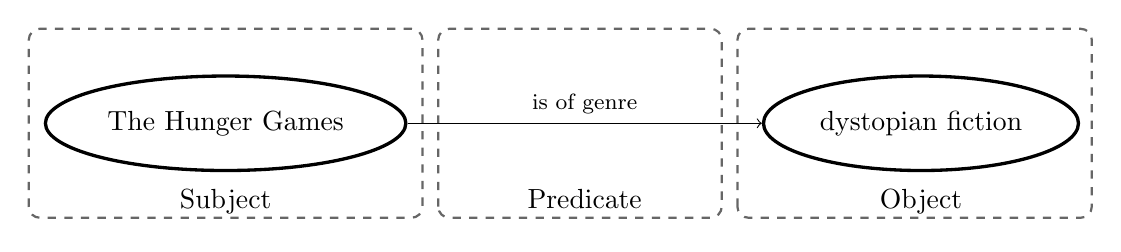
\begin{tikzpicture}[
        vertex/.style={ellipse,draw=black,very thick, minimum width = 4cm, minimum height = 1.2cm},
        predicate/.style = {font=\footnotesize}
    ]
    \node[vertex,label={[yshift=-1.9cm]Subject}] (thg) {The Hunger Games};
    \node[vertex,label={[yshift=-1.9cm]Object}] (dystopian) [right=4.5cm of thg] {dystopian fiction};

    \filldraw[thick,fill=none,draw=black!60,dashed, rounded corners] (-2.5,-1.2) rectangle (2.5,1.2);
    \filldraw[thick,fill=none,draw=black!60,dashed, rounded corners] (2.7,-1.2) rectangle (6.3,1.2);
    \filldraw[thick,fill=none,draw=black!60,dashed, rounded corners] (6.5,-1.2) rectangle (11,1.2);

    \path[-to] (thg) edge node[predicate,above,label={[yshift=-1.7cm]Predicate}] {is of genre} (dystopian);
\end{tikzpicture}
\end{document}